\documentclass{article}
\renewcommand{\theequation}{\arabic{equation}}

% ready for submission
\usepackage[preprint]{nips_2018}

% to compile a preprint version, e.g., for submission to arXiv, add
% add the [preprint] option:
% \usepackage[preprint]{nips_2018}

% to compile a camera-ready version, add the [final] option, e.g.:
% \usepackage[final]{nips_2018}

% to avoid loading the natbib package, add option nonatbib:
% \usepackage[nonatbib]{nips_2018}

\usepackage[utf8]{inputenc} % allow utf-8 input
\usepackage[T1]{fontenc}    % use 8-bit T1 fonts
\usepackage{hyperref}       % hyperlinks
\usepackage{url}            % simple URL typesetting
\usepackage{booktabs}       % professional-quality tables
\usepackage{amsfonts}       % blackboard math symbols
\usepackage{nicefrac}       % compact symbols for 1/2, etc.
\usepackage{microtype}      % microtypography
\usepackage{tikz}
\usepackage{standalone}

\title{Diagnet: A Fast New Recurrent Neural Network Architecture}
 
\author{
Thomas Lahore\\
\texttt{tom.lahore@gmail.com}\\
\And
Morgan Weaver\\
\texttt{morganjweaver@gmail.com}
}

\begin{document}
\maketitle
\begin{abstract}

  Recurrent neural networks have long been plagued by the vanishing and exploding gradient problems and limited performance over increasing time steps. We propose Diagnet, a novel RNN design which incorporates architectural and process-oriented elements which, in combination, greatly increase the stability and quality of the error gradient. We demonstrate in a variety of benchmarking tasks that learning becomes possible with delays of up to 10,000 time steps, representing substantial gains over existing RNN designs.  Diagnet’s architecture relies upon three core features: 1) A single layer of segregated recurrent units which are self-connected 2) The absolute value function (an unbounded norm-preserving idempotent nonlinearity), and 3) Application of constraints in both recurrent parameter weights and gradient norms, which tightly control the exploding gradient problem.  Despite the segregated and simplistic nature of Diagnet's recurrent units, significant performance improvement is seen in the 1000-example, weakly-supervised version of the bAbI tasks as compared to Long Short Term Memory. Diagnet scores higher in testing on 15 out of the 20 tasks, by margins of 3-30\% accuracy, while enabling the use of significantly more hidden neurons than fully-connected RNNs. 

%  The abstract paragraph should be indented \nicefrac{1}{2}~inch
%  (3~picas) on both the left- and right-hand margins. Use 10~point
%  type, with a vertical spacing (leading) of 11~points.  The word
%  \textbf{Abstract} must be centered, bold, and in point size 12. Two
%  line spaces precede the abstract. The abstract must be limited to
%  one paragraph.
\end{abstract}

\section{Introduction}

%NIPS requires electronic submissions.  The electronic submission site
%is
%\begin{center}
%  \url{https://cmt.research.microsoft.com/NIPS2018/}
%\end{center}
%
%Please read the instructions below carefully and follow them faithfully.
Recurrent neural networks represent one of the most important deep learning architectures in current use.  They are increasingly being used for many tasks, such as time series prediction [REF], unsegmented, connected handwriting recognition [REF], large-vocabulary speech recognition [REF], modeling chaotic phenomena [REF], language modeling and machine translation [REF], robot control [REF], Protein Homology Detection [REF].
      
We are interested in addressing two widely-cited [REF] pain points of RNN performance.  The first being the vanishing and exploding gradient problem [REF], and the second being performance over increasing time steps [REF].  We address these issues by implementing three as kjfhakdf that have not yet been exibited in combination in neural net design. 
What we found Results were...impressive

In the following paper, we present a brief outline of foundational work in the problem space to contextualize Diagnet’s emergence in RNN design.  Then, we present a discussion of the architecture and mechanisms of Diagnet, along with a useful visual tool for building an intuitive understanding of Diagnet’s units and their behavior.  Next we present a series of common benchmarking tasks, the results of each task, and finally conclude with a discussion of Diagnet’s performance and behavior based on experimental results.  We hope to offer an interesting and powerful new tool for sequence modeling in our introduction of Diagnet, while laying the groundwork for further exploration, architectural innovation, and interaction with the ML community.

%\paragraph{New preprint option for 2018}
%If you wish to post a preprint of your work online, e.g., on arXiv,
%using the NIPS style, please use the \verb+preprint+ option. This will
%create a nonanonymized version of your work with the text
%``Preprint. Work in progress.''  in the footer. This version may be
%distributed as you see fit. Please \textbf{do not} use the
%\verb+final+ option, which should \textbf{only} be used for papers
%accepted to NIPS.
%
%At submission time, please omit the \verb+final+ and \verb+preprint+
%options. This will anonymize your submission and add line numbers to aid
%review. Please do \emph{not} refer to these line numbers in your paper
%as they will be removed during generation of camera-ready copies.
%
%The file \verb+nips_2018.tex+ may be used as a ``shell'' for writing
%your paper. All you have to do is replace the author, title, abstract,
%and text of the paper with your own.
%
%The formatting instructions contained in these style files are
%summarized in Sections \ref{gen_inst}, \ref{headings}, and
%\ref{others} below.

\section{Previous Work}
\label{gen_inst}
It is important to consider a new deep learning architecture with an awareness of existing models.  We offer a brief and by no means comprehensive overview of existing RNN designs herein.  
Some of the earliest work consists of Hopfield Networks, developed by Hopfield in 1982.  Subsequently, Schmidhuber [REF] developed the Neural History Compressor (1993) and was able to preserve information over time steps, while compressing information.  In 1991 Fallman developed the Recurrent Cascade Correlation Algorithm \citet{Fahlman1990TheRC}, in which a single, previously trained hidden unit is added to the network at a time, with incoming weights frozen as the incoming unit is connected in a feed-forward manner with the previous output units. Each new hidden neuron must be maximally correlated with current remaining error per step.  Now make recurrent: each neuron has single link to self.  Rinse n repeat algo; truncated backprop at the time bc feasible.  At time, proved not useful for certain grammars like seq parity (using saturating, not abs val fxn). First paper T knows of where neuron self-connected. (IndRNN first layer is the same)
In 1997, Hochreiter and Schmidhuber introduced Long Short-Term Memory (LSTM), which sought to address the vanishing and exploding gradient problem with constant error flow through specialized units in addition to multiplicative gated memory units, resulting in more efficient storage of information at little computational cost.  
GRU (2014)-just ref it, no significant influence
IRNN (2015)-identity RNN--HINTON, recurrent neurons are relus, init at ID matrix. 2 big ideas. Prob: not used bc unstable, need right params.  Good init results > LSTM simpler architecture. Init at ID matrix was the big idea (unitary matrix) Diagnet too--but off-dig values can't ever be anything but 0; diag are all 1 fast Hadamard product instead of tiresome n\^2.
SCRN (2015)--diagonal entries connected constrained to 1 or a min val, so self-recurrent.  Recognizing value of separate way of handling given recurrent unit connections to self.  Better task results but not less complex computationally. Higher quality learning process.
uRNN (2015)-Bengio et al.  addresses vanishing gradient prob, not exploding.  Transition matrix is unitary.  Enorced.  Complex numbers, etc. Decent results.
DizzyRNN (2016)-abs val. weight matrix unitary transformations, broken into pairs of 2, use 2d rotations. reasonable results. 1-2 tasks 
IndRNN  (2018)--uses self-connection in first layer, loses much efficiency.  Many-to-many connection. Very expensive.  Uses relu for non-linearity rather than our absval.  
Gradient clipping--2 uses here--1)take norm of gradient over all params and limit to N; throw away.  If larger, rescale.  2) Gradients on indiv params, scale down if exceeds limit.  Lossy, loses vector direction information. Directionality is better preserved in this multi-targeted approach. First pass then prune outliers.    

Besides architectural innovations, progress has been made in controlling the gradient directly.

Clipped Gradients (Paskanu, Mikolov, Bengio)

Make a chart of architectures vs features?
Make a feature matrix showing what overlaps the various solutions have? That might be of more interest, and faster than simply talking about all of them individually. We can still cite them.

\section{Architecture}
\label{headings}
\begin{figure}
  \centering
  \includestandalone[scale=0.5]{figures/diagnet1}
  \caption{Figure showing nice diagram of the architecture.}
\end{figure}

Densely connected from input to hidden layer.
Only a single, “shallow” hidden layer.
Hidden layer has no biases.
Hidden layer is recurrently connected by a diagonal matrix; thus every hidden neuron is solely recurrently self-connected.
Self connections of hidden neurons are clamped to lie in the range [-1.0, 1.0]
Self connections of hidden neurons are initialized at 1.0.
Each hidden neuron makes use of the absolute value function as a nonlinearity.
There are no gates* (see “poor man’s gate” section later for an architectural variant)
Densely connected from hidden layer to output
%All headings should be lower case (except for first word and proper
%nouns), flush left, and bold.

%First-level headings should be in 12-point type.

\subsection{Absolute Value Function}

The absolute value function was chosen because it is has a number of desirable properties: 

\begin{itemize}
\item Nonlinear: This is a requirement for useful computations to be possible
\item Unbounded: Can I make an argument for why this is an important thing? Something somthing Turing-complete?
\item Idempotent: This aspect of stability may allow for long term, high precision storage of information without specialized architectural design
\item (Almost) Everywhere differentiable: It is (almost) everywhere differentiable, with unit-length derivatives of either -1 or 1
\item Norm-preserving: It is norm-preserving, both for each individual component of the vector, and also for the vector as a whole.
The absolute value function cannot, by itself, cause gradients to explode, nor vanish
\end{itemize}


\begin{figure}[hbtp]
\centering
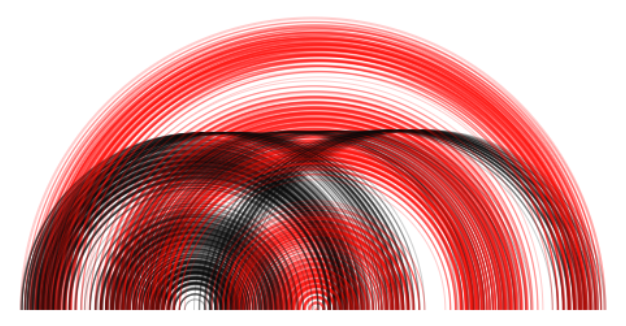
\includegraphics[scale=0.25]{images/state-space2.png}
\caption{Absolute value dynamics}
\end{figure}

Generic restatements about why norm preservation is important when training recurrent neural networks.

LSTM and GRU preserve the gradient over time by mostly avoiding the direct application of nonlinearities as much as possible. ResNet is intuitively similar in this sense. (TODO: Highway networks?) However, it is likely the case that many potentially useful algorithms or dynamical behaviors require the application of a long sequence of nonlinear transformations, rather than simply preserving a small number of computations/transformations over extensive spans of time.

One toy problem that requires a long, unbroken chain of nonlinear transformations is sequential parity, which will be visited below (and which LSTM and GRU are completely unable to solve for T > 10.)

Others [REF] [REF] have experimented with using the absolute value function in RNNs, but overall this is a largely unexplored activation function.
 
We speculate that it has not received much attention as of yet, because very special care must be taken to control the spectral radius of the recurrent matrix.

Something about absolute value function being the only continuous norm preserving non-linearity (is that true?).

\subsection{Constraints}

Postulate that absolute value function hasn’t been explored much, particularly for recurrent neural nets, because without the proper constraints, its values tend to rapidly blow up.


\subsubsection{Limited [-1, 1] range}
Important to have these constraints, otherwise blows up.
This is an extremely simple way of limiting the spectral radius of the matrix.
In fact (double check) because of the constrained structure, these “recurrent factors” can straightforwardly tell us the singular values, eigenvalues, spectral radius of the linear transformation. (I think the fact that we use no biases helps because it remains linear rather than affine.)

Mention that on some tasks, it often ends up using very different “signatures” of recurrent factor values.

Mention importance of initializing to 1.0 here? Different section?
\subsubsection{Two complementary types of gradient clipping}

Some form of gradient clipping is standard practice for RNNs [REF], but to our knowledge, this is the first application of both global and localized clipping (and it is important to do both!)

Appears to be critical to limit the size of the overall norm of the gradient, particularly for some of the really long-delay tasks.

Critical to do a combination of both global and local norm clipping. Either alone is insufficient.
\subsection{Architectural variations}
\subsubsection{Input masking (“Poor man’s gate”)}

\begin{equation}
  h_t := | u \circ h_{t-1} + W\sigma (Vx_t)) |
\end{equation}

% \[h_t = | u \circ h_{t-1} + W\sigma (Vx_t)) |\]

Because the recurrent layer uses no gating mechanism, it can sometimes be useful to have an extra feed forward hidden layer that can learn to selectively ignore certain inputs. In the pathological sequence problems, we have chosen to use ReLU units, because of their hard stop at zero.
This is necessary for all of the “pathological” problems.
“Poor man’s gate” can only mask information that is immediately identifiable as not useful; makes use of no prior contextual information.

%\paragraph{Paragraphs}
%
%There is also a \verb+\paragraph+ command available, which sets the
%heading in bold, flush left, and inline with the text, with the
%heading followed by 1\,em of space.
%
\section{Experiments}
\label{others}
Experimental settings, like learning rates, cooling schedules, hidden layer sizes, etc..

\begin{table}[ht]
\caption{Hooray for a random table} % title of Table
\centering % used for centering table
\begin{tabular}{c c c c} % centered columns (4 columns)
\hline\hline %inserts double horizontal lines
Case & Method\#1 & Method\#2 & Method\#3 \\ [0.5ex] % inserts table
%heading
\hline % inserts single horizontal line
1 & 50 & 837 & 970 \\ % inserting body of the table
2 & 47 & 877 & 230 \\
3 & 31 & 25 & 415 \\
4 & 35 & 144 & 2356 \\
5 & 45 & 300 & 556 \\ [1ex] % [1ex] adds vertical space
\hline %inserts single line
\end{tabular}
\label{table:nonlin} % is used to refer this table in the text
\end{table}

All experiments use the following settings:

RMSprop*, with a learning rate of 0.001
Recurrent parameters are all initialized to 1.0
Feed forward parameters use Xavier’s initialization [REF]
Global gradient norm clipped at 30.0
Per-parameter gradients clipped at [-1.0, 1.0]

Initialize all recurrent factors to 1.0
Derivative clipping
Weight initialization scheme
*Try with mini-batches
Hidden layer sizes
Poor-man’s gate sizes

Maybe make a table of these things for all the experiments? That would be pleasant to read

\subsection{Facebook bAbI Question-Answering}

bAbI is a set of 20 synthetic natural language understanding tasks created by \citet{2015arXiv150205698W}. Each task has been designed to test for particular logical and reasoning capabilities, such as induction, deduction, chaining of facts, temporal ordering of events, as well as others. It is suggested that solving these "toy" problems is a necessary (although not sufficient) precondition to the development of truly intelligent systems.

In the paper, it was shown that a plain LSTM network was unable to solve any of the 20 tasks, where success had been defined as attaining an accuracy of 95\% or more.

The initial, significant improvement over a plain RNN baseline was in the form of MemNNs, previously introduced in [REF]. And since then a number of new techniques have been successfully applied to bAbI, generally falling into two overall domains: augmented memories, and attentional mechanisms.

Augmented memories are a family of approaches that involve fitting a neural network (generally a recurrent one) with an "external" - and differently structured - form of memory. These external memory stores are generally more inspired by computer science than biology, and include concepts such as content addressable memory, random access memory, stacks, queues, Turing tapes, cellular automata, etc.. Almost all external memories make use of fully differentiable read and write mechanisms, although there are a few notable exceptions that are discrete in nature; requiring reinforcement learning rather than pure backpropagation in order to train.

The other significant family of approaches involve attentional mechanisms. Attentional mechanisms have met with great recent success, particularly in the domain of machine translation. Rather than having the neural network improve its ability to store information initially, attentional mechanisms all the model to go back over the sequential history of its inputs, often multiple times, conditioned on the type of output that is expected. In the case of machine translation, that conditioning will be driven by the next word in the sentence it is translating combined with what it has already produced. In the case of natural language understanding, it is the question being asked that conditions the attention to the relevant subset of facts in the preceding material. In essence, attention allows models to selectively reread do further processing on what has already been seen.

Diagnet does none of this, yet. But future experiments will undoubtedly involve memory enhancing alterations, with Diagnet as the core "controller" of the architecture. 



%TODO: how to make sure this table appears after the subsection?
\begin{table}
\caption{Example from bAbI problem set}
\centering
\begin{tabular}{|l|l|l|}
\hline
Fact & Question & Answer \\
\hline
Mary moved to the bathroom. & & \\
John went to the hallway. & & \\
 & Where is Mary? & bathroom \\
Daniel went back to the hallway. & & \\
Sandra moved to the garden. & & \\
 & Where is Daniel? & hallway \\
John moved to the office. & & \\
Sandra journeyed to the bathroom. & & \\
& Where is Daniel? & hallway \\
Mary moved to the hallway. & & \\
Daniel travelled to the office. & & \\
& Where is Daniel? & office \\
John went back to the garden. & & \\
John moved to the bedroom. & & \\
& Where is Sandra? & bathroom \\
\hline
\end{tabular}
\end{table}

In the accompanying paper, Weston et al introduce Memory Networks in order to overcome many of the shortcomings of a plain LSTM network. 

Additionally, it has been found that adding attentional mechanisms to input history has resulted in significantly improved performance.

ADD MORE STUFF ABOUT THAT HERE

Note that in this work we are not comparing Diagnet directly to any of the aforementioned “augmented” neural architectures. Instead, we demonstrate that Diagnet significantly outperforms LSTM and GRU on many of these 20 tasks, even despite using a much simpler and computationally efficient internal architecture.

\begin{table}

\centering
\caption{bAbI test set accuracies}
\begin{tabular}{|l|r|r|r|}
\hline
Task & LSTM & Diagnet & +/- \\
\hline
Single Supporting Fact & 50 & \textbf{72.1} & +22.1 \\
Two Supporting Facts & 20 & \textbf{31.8} & +11.8 \\
Three Supporting Facts & 20 & \textbf{32.4} & +12.4 \\
Two Arg. Relations & 61 & \textbf{98.9} & +37.9 \\
Three Arg. Relations & 70 & \textbf{82.4} & +12.4 \\
Yes/No Questions & 48 & \textbf{72.4} & +24.4 \\
Counting & 49 & \textbf{82.1} & +33.1 \\
Lists/Sets & 45 & \textbf{75.1} & +30.1 \\
Simple Negation & 64 & \textbf{77}.0 & +13.0 \\
Indefinite Knowledge & 44 & \textbf{66.8} & +22.8 \\
Basic Coreference & 72 & \textbf{81.3} & +9.3 \\
Conjunction & 74 & \textbf{90.4} & +6.4 \\
Compound Coreference & 94 & \textbf{94.2} & +0.2 \\
Time Reasoning & 27 & \textbf{39.6} & +12.6 \\
Basic Deduction & 21 & \textbf{49.1} & +28.1 \\
Basic Induction & 23 & \textbf{46.5} & +23.5 \\
Positional Reasoning & \textbf{51} & \textcolor{red}{50.1} & -0.9 \\
Size Reasoning & 52 & \textbf{92.0} & +40.0 \\
Path Finding & 8 & \textbf{12.4} & +4.4 \\
Agent's Motivations & 91 & \textbf{96.3} & +5.3 \\
\hline

\end{tabular}

\end{table}

As far as we are aware, these are the strongest results to date using a “plain” neural neural architecture on the 1k, weakly supervised version of the bAbI tasks.

This suggests that Diagnet may represent 

\section{Discussion}
\subsection{Future Work}
Diagnet's architecture suggests many avenues for additional tasks and performance-enhancing modifications.  Its segregated unit design is ideal for parallelization, and we have yet to tap its potential for GPU operations.  Another intuitive addition would be to include an attentional mechanism or memory augmentation, which we leave to future publications.  
As RNNs have historically been utilized with great success in NLP tasks, we intend to continue exploring Diagnet's capabilities in this problem space.  Another area in which complex long-range sequences are of great interest is computational genomics. The roughly 1.5-gigabytes of information in the human genome may benefit from an RNN architecture supporting wider hidden layers.  

\section{Conclusion}
Here we outline the features, mechanisms, and benchmarking performance of Diagnet. Results were robust over a variety of tasks, most notably in bAbI question-answering tasks, where Diagnet’s accuracy scores showed up to 36\% percent improvement over existing architectures such as LSTM and GRU.  While memory augmentation and attentional mechanisms offer clear advantages as architectural additions, we choose to focus on the core RNN functionality in this paper.  Future work may incorporate attentional mechanisms, memory augmentation, and additional task spaces such as semantic embeddings, genetic sequencing, and computer vision.  Diagnet’s novel architecture offers great flexibility in hidden layering, and number of steps in various memory tasks, as well as potential for distributed computing.  Due to the fact that Diagnet does not have gating mechanisms in its current iteration, it is largely input-driven, and tends to perform best in tasks where an output sequence is expected after arbitrary delays. The work presented here represents a first glance at Diagnet’s mechanisms and potential, which the authors hope to expand in future work. 


%The \verb+natbib+ package will be loaded for you by default.
%Citations may be author/year or numeric, as long as you maintain
%internal consistency.  As to the format of the references themselves,
%any style is acceptable as long as it is used consistently.

%The documentation for \verb+natbib+ may be found at
%\begin{center}
%  \url{http://mirrors.ctan.org/macros/latex/contrib/natbib/natnotes.pdf}
%\end{center}
%Of note is the command \verb+\citet+, which produces citations
%appropriate for use in inline text.  For example,
%\begin{verbatim}
%   \citet{hasselmo} investigated\dots
%\end{verbatim}
%produces
%\begin{quote}
%  Hasselmo, et al.\ (1995) investigated\dots
%\end{quote}
%
%If you wish to load the \verb+natbib+ package with options, you may
%add the following before loading the \verb+nips_2018+ package:
%\begin{verbatim}
%   \PassOptionsToPackage{options}{natbib}
%\end{verbatim}
%
%If \verb+natbib+ clashes with another package you load, you can add
%the optional argument \verb+nonatbib+ when loading the style file:
%\begin{verbatim}
%   \usepackage[nonatbib]{nips_2018}
%\end{verbatim}
%
%As submission is double blind, refer to your own published work in the
%third person. That is, use ``In the previous work of Jones et
%al.\ [4],'' not ``In our previous work [4].'' If you cite your other
%papers that are not widely available (e.g., a journal paper under
%review), use  author names in the citation, e.g., an author
%of the form ``A.\ Anonymous.''
%
%\subsection{Footnotes}
%
%Footnotes should be used sparingly.  If you do require a footnote,
%indicate footnotes with a number\footnote{Sample of the first
%  footnote.} in the text. Place the footnotes at the bottom of the
%page on which they appear.  Precede the footnote with a horizontal
%rule of 2~inches (12~picas).
%
%Note that footnotes are properly typeset \emph{after} punctuation
%marks.\footnote{As in this example.}
%
%\subsection{Figures}
%
%\begin{figure}
%  \centering
%  \fbox{\rule[-.5cm]{0cm}{4cm} \rule[-.5cm]{4cm}{0cm}}
%  \caption{Figure showing nice diagram of the architecture.}
%\end{figure}
%
%All artwork must be neat, clean, and legible. Lines should be dark
%enough for purposes of reproduction. The figure number and caption
%always appear after the figure. Place one line space before the figure
%caption and one line space after the figure. The figure caption should
%be lower case (except for first word and proper nouns); figures are
%numbered consecutively.
%
%You may use color figures.  However, it is best for the figure
%captions and the paper body to be legible if the paper is printed in
%either black/white or in color.
%
%\subsection{Tables}
%
%All tables must be centered, neat, clean and legible.  The table
%number and title always appear before the table.  See
%Table~\ref{sample-table}.
%
%Place one line space before the table title, one line space after the
%table title, and one line space after the table. The table title must
%be lower case (except for first word and proper nouns); tables are
%numbered consecutively.
%
%Note that publication-quality tables \emph{do not contain vertical
%  rules.} We strongly suggest the use of the \verb+booktabs+ package,
%which allows for typesetting high-quality, professional tables:
%\begin{center}
%  \url{https://www.ctan.org/pkg/booktabs}
%\end{center}
%This package was used to typeset Table~\ref{sample-table}.
%
%\begin{table}
%  \caption{Sample table title}
%  \label{sample-table}
%  \centering
%  \begin{tabular}{lll}
%    \toprule
%    \multicolumn{2}{c}{Part}                   \\
%    \cmidrule(r){1-2}
%    Name     & Description     & Size ($\mu$m) \\
%    \midrule
%    Dendrite & Input terminal  & $\sim$100     \\
%    Axon     & Output terminal & $\sim$10      \\
%    Soma     & Cell body       & up to $10^6$  \\
%    \bottomrule
%  \end{tabular}
%\end{table}
%
%\section{Final instructions}
%
%Do not change any aspects of the formatting parameters in the style
%files.  In particular, do not modify the width or length of the
%rectangle the text should fit into, and do not change font sizes
%(except perhaps in the \textbf{References} section; see below). Please
%note that pages should be numbered.
%
%\section{Preparing PDF files}
%
%Please prepare submission files with paper size ``US Letter,'' and
%not, for example, ``A4.''
%
%Fonts were the main cause of problems in the past years. Your PDF file
%must only contain Type 1 or Embedded TrueType fonts. Here are a few
%instructions to achieve this.
%
%\begin{itemize}
%
%\item You should directly generate PDF files using \verb+pdflatex+.
%
%\item You can check which fonts a PDF files uses.  In Acrobat Reader,
%  select the menu Files$>$Document Properties$>$Fonts and select Show
%  All Fonts. You can also use the program \verb+pdffonts+ which comes
%  with \verb+xpdf+ and is available out-of-the-box on most Linux
%  machines.
%
%\item The IEEE has recommendations for generating PDF files whose
%  fonts are also acceptable for NIPS. Please see
%  \url{http://www.emfield.org/icuwb2010/downloads/IEEE-PDF-SpecV32.pdf}
%
%\item \verb+xfig+ "patterned" shapes are implemented with bitmap
%  fonts.  Use "solid" shapes instead.
%
%\item The \verb+\bbold+ package almost always uses bitmap fonts.  You
%  should use the equivalent AMS Fonts:
%\begin{verbatim}
%   \usepackage{amsfonts}
%\end{verbatim}
%followed by, e.g., \verb+\mathbb{R}+, \verb+\mathbb{N}+, or
%\verb+\mathbb{C}+ for $\mathbb{R}$, $\mathbb{N}$ or $\mathbb{C}$.  You
%can also use the following workaround for reals, natural and complex:
%\begin{verbatim}
%   \newcommand{\RR}{I\!\!R} %real numbers
%   \newcommand{\Nat}{I\!\!N} %natural numbers
%   \newcommand{\CC}{I\!\!\!\!C} %complex numbers
%\end{verbatim}
%Note that \verb+amsfonts+ is automatically loaded by the
%\verb+amssymb+ package.
%
%\end{itemize}
%
%If your file contains type 3 fonts or non embedded TrueType fonts, we
%will ask you to fix it.
%
%\subsection{Margins in \LaTeX{}}
%
%Most of the margin problems come from figures positioned by hand using
%\verb+\special+ or other commands. We suggest using the command
%\verb+\includegraphics+ from the \verb+graphicx+ package. Always
%specify the figure width as a multiple of the line width as in the
%example below:
%\begin{verbatim}
%   \usepackage[pdftex]{graphicx} ...
%   \includegraphics[width=0.8\linewidth]{myfile.pdf}
%\end{verbatim}
%See Section 4.4 in the graphics bundle documentation
%(\url{http://mirrors.ctan.org/macros/latex/required/graphics/grfguide.pdf})
%
%A number of width problems arise when \LaTeX{} cannot properly
%hyphenate a line. Please give LaTeX hyphenation hints using the
%\verb+\-+ command when necessary.

\subsubsection*{Acknowledgments}

The authors would like to express their gratitude to their sponsor .

%\section*{References}

\bibliographystyle{plainnat}
\bibliography{refs}


%References follow the acknowledgments. Use unnumbered first-level
%heading for the references. Any choice of citation style is acceptable
%as long as you are consistent. It is permissible to reduce the font
%size to \verb+small+ (9 point) when listing the references. {\bf
%  Remember that you can use more than eight pages as long as the
%  additional pages contain \emph{only} cited references.}
%\medskip
%
%\small
%
%[1] Alexander, J.A.\ \& Mozer, M.C.\ (1995) Template-based algorithms
%for connectionist rule extraction. In G.\ Tesauro, D.S.\ Touretzky and
%T.K.\ Leen (eds.), {\it Advances in Neural Information Processing
%  Systems 7}, pp.\ 609--616. Cambridge, MA: MIT Press.
%
%[2] Bower, J.M.\ \& Beeman, D.\ (1995) {\it The Book of GENESIS:
%  Exploring Realistic Neural Models with the GEneral NEural SImulation
%  System.}  New York: TELOS/Springer--Verlag.
%
%[3] Hasselmo, M.E., Schnell, E.\ \& Barkai, E.\ (1995) Dynamics of
%learning and recall at excitatory recurrent synapses and cholinergic
%modulation in rat hippocampal region CA3. {\it Journal of
%  Neuroscience} {\bf 15}(7):5249-5262.

\end{document}
